%                                                                 aa.dem
% AA vers. 8.2, LaTeX class for Astronomy & Astrophysics
% demonstration file
%                                                       (c) EDP Sciences
%-----------------------------------------------------------------------
%
%\documentclass[referee]{aa} % for a referee version
%\documentclass[onecolumn]{aa} % for a paper on 1 column  
%\documentclass[longauth]{aa} % for the long lists of affiliations 
%\documentclass[rnote]{aa} % for the research notes
%\documentclass[letter]{aa} % for the letters 
%\documentclass[bibyear]{aa} % if the references are not structured 
% according to the author-year natbib style

%%%%%%%%%%%%%%%%%%%%%%%%%%%%%%%%%%%%%%%%%%%%%%%%%%%%%%%%%%%%%%%%%%%%%%%%%%%%
\documentclass{aa}    %% Astronomy & Astrophysics style class aa.cls v8.2

\usepackage{graphicx,url,twoopt,natbib}
\usepackage[varg]{txfonts}           %% A&A font choice

\usepackage{pdfcomment}              %% for popup acronym meanings
\usepackage{acronym}                 %% for popup acronym meanings




\usepackage{color,hyperref}
\definecolor{linkcolor}{rgb}{0,0,0.5}
\hypersetup{colorlinks=true,
					linkcolor=linkcolor, 
					citecolor=linkcolor,
                    filecolor=linkcolor, 
                    urlcolor=linkcolor}



\bibpunct{(}{)}{;}{a}{}{,}    %% natbib cite format used by A&A and ApJ

%\pagestyle{plain}     %% undo the fancy A&A pagestyle 

%% Add commands to add a note or link to a reference
\makeatletter
\newcommand{\bibnote}[2]{\@namedef{#1note}{#2}}
\newcommand{\biblink}[2]{\@namedef{#1link}{#2}}
\makeatother




% % Labels
\newcommand{\figref}[1]{\ref{fig:#1}}
\newcommand{\Fig}[1]{\figurename~\figref{#1}}
\newcommand{\fig}[1]{\Fig{#1}}
\newcommand{\figlabel}[1]{\label{fig:#1}}
\newcommand{\Tab}[1]{Table~\ref{tab:#1}}
\newcommand{\tab}[1]{\Tab{#1}}
\newcommand{\tablabel}[1]{\label{tab:#1}}
\newcommand{\Eq}[1]{Equation~(\ref{eq:#1})}
\newcommand{\eq}[1]{\Eq{#1}}
\newcommand{\eqalt}[1]{Equation~\ref{eq:#1}}
\newcommand{\eqlabel}[1]{\label{eq:#1}}
\newcommand{\sectionname}{Section}
\newcommand{\Sect}[1]{\sectionname~\ref{sect:#1}}
\newcommand{\sect}[1]{\Sect{#1}}
\newcommand{\sectalt}[1]{\ref{sect:#1}}
\newcommand{\App}[1]{Appendix~\ref{sect:#1}}
\newcommand{\app}[1]{\App{#1}}
\newcommand{\sectlabel}[1]{\label{sect:#1}}



%% Spectral species

\newcommand{\lya}{Ly$\alpha$} 
\newcommand{\lyb}{Ly$\beta$} 
\newcommand{\hb}{H$\beta$} 
\newcommand{\ha}{H$\alpha$} 
\newcommand{\oi}{[\ion{O}{i}]} 
\newcommand{\sii}{[\ion{S}{ii}]} 
\newcommand{\oii}{[\ion{O}{ii}]} 
\newcommand{\oiii}{[\ion{O}{iii}]}
\newcommand{\nii}{[\ion{N}{ii}]} 
\newcommand{\feii}{[\ion{Fe}{ii}]} 
\newcommand{\civ}{\ion{C}{iv}} 
\newcommand{\mgii}{\ion{Mg}{ii}} 

%% Useful shortcuts
\newcommand{\fluxunit}{erg s$^{-1}$ cm$^{-2}$ \AA$^{-1}$} 

\newcommand{\myemail}{jselsing@dark-cosmology.dk}


% TO DOS
\newcommand{\todo}[3]{{\color{#2}\emph{#1}: #3}}
\newcommand{\jstodo}[1]{\todo{TODO }{green}{#1}}
\newcommand{\qtodo}[1]{\todo{Question}{red}{#1}}



%%%%%%%%%%%%%%%%%%%%%%%%%%%%%%%%%%%%%%%%%%%%%%%%%%%%%%%%%%%%%%%%%%%%%%%%%%%





\begin{document}  
\title{An X-shooter composite of bright 1<z<2 quasars from UV to Infrared \thanks{Based on observations made with telescopes at the European Southern Observatory at LaSilla/Paranal, Chile under program 090.A-0147(A).}}

\titlerunning{X-shooter Quasar Composite}


\author{J. Selsing\inst{1}, J.~P.~U. Fynbo\inst{1}, L. Christensen\inst{1}, J.-K. Krogager\inst{1}
		  }

          

\authorrunning{J. Selsing et al.}


\institute{
	Dark Cosmology Centre, Niels Bohr Institute, University of Copenhagen, Juliane Maries Vej 30, 2100 Copenhagen, Denmark. %\and
		 }

             
\date{Draft version, February, 2015} %{Received September 15, 1996; accepted March 16, 1997}

% \abstract{}{}{}{}{} 
% 5 {} token are mandatory
 
\abstract{
\jstodo{The abstract is taken from the proposal and should be adapted to the paper.}
QSO templates are important both for QSO physics and for projects using QSOs as probes. However, the current most widely used QSO template, namely the SDSS composite QSO spectrum of Vanden Berk et al. (2001) suffers from significant host galaxy contamination redwards of 5000\AA in the restframe. At these wavelenghts the SDSS template is based on intrinsically faint, low-redshift QSOs. We here propose to build a composite QSO spectrum for bright blue QSOs without this problem using X-shooter GTO time. With X-shooter we can target bright SDSS QSOs in the redshift range $1 < z < 2.3$ and hence build a composite spectrum covering the full range from Ly$\alpha$ to 8500\AA in the restframe without significant host galaxy contamination.  

}{}{}{}{}




\keywords{Quasars: general --- quasars: composite spectrum --- quasars: host galaxy}

\maketitle
%
%________________________________________________________________


%%%%%%%%%%%%%%%%%%%%%%%%%%%%%%%%%%%%%%%%%%%%%%%%%%%%%%%%%%%%%%%%%%%%%%%%%%%%
\section{Introduction}     \sectlabel{introduction}
%%%%%%%%%%%%%%%%%%%%%%%%%%%%%%%%%%%%%%%%%%%%%%%%%%%%%%%%%%%%%%%%%%%%%%%%%%%%
%
%The optical-to-ultraviolet emission mechanism of quasars are by now quite well understood \citep{Elvis1994}. A supermassive black hole at the center of a galaxy is surrounded by a hot accretion disc which emits a featureless thermal continuum. The central continuum photoionizes a region of hot clouds, and further out, cold clouds which gives rise to lines with both broad and narrow components \citep{Elvis2001}.  Varying conditions in the clouds ensure that each ionic species have optimal conditions to produce line emission \citep{Baldwin1995}. Despite the apparent different conditions in which the emission arises, the overall shape of most quasar spectra look similar {\color{red} Reference needed}. The remarkable uniformity of the average spectral properties across luminosity and redshift indicate very similar underlying physical mechanisms which can be understood in terms of Eigenvector 1 (\citep{Boroson1992}; \cite{Francis1992}) where the Eddington ratio drives the relative strength of the lines and orientation effects influences the observed kinematics of the lines \citep{Shen2014a} accounting for the majority of the inter-quasar variation. This means that the accretion rate and the mass of the black hole largely determines the spectral appearance of a given quasar. 
%
%Template spectra are useful for a wide range of purposes, e.g., the detection of features that are too weak to be detected in individual spectra, identification of objects that differ from the mean, etc. Examples of such composite spectra include template spectra of various classes of galaxies (\cite{Shapley2003}; \cite{Dobos2012}), QSOs (\cite{CristianiS.andVio1990}; \cite{Boyle1990}; \cite{Francis1991}; \cite{Zheng1997} \cite{Brotherton2000}; \cite{VandenBerk2001}; \cite{Telfer2002}; \cite{Richards2006}; \cite{Glikman2006}) and GRB afterglows \citep{Christensen2011}. In particular, QSO composite spectra have been studied and discussed intensively since the first papers in the early 1990ies.
%
%When investigating dust in quasars, templates can be used to determine the amount of extinction by artificially reddening to match an observed spectrum (\cite{Glikman2007}; \cite{Urrutia2009}; \cite{Wang2012}; \cite{Fynbo2013}; \cite{Krogager2015}). The amount of extinction inferred will depend on what kind of dust is assumed,  which for quasars has been found to be SMC-like (\cite{Richards2003}; \cite{Hopkins2004}),  the parametrization chosen (\cite{Gordon2003};\cite{Fitzpatrick2005} ) and the template spectrum used. 
%
%The wavelength coverage of a single instrument is always limited and therefore templates from different telescopes cover different regions. The redshift distribution of quasars are exploited to extend the wavelength coverage of a single instrument while covering bad atmospheric windows, but because of the this, different parts of the template will be attributed to different redshifts. Several instruments can be combined to extend the wavelength coverage of a single template as is done in \citep{Glikman2006} where SDSS \citep{Gunn2006} and IRTF, SpeX \citep{Rayner2003} spectra are combined to cover the range from 2700 \AA~ to 37000 \AA, or several templates can be combined to cover regions of interest as done in \citep{Zhou2010} where the template of \citep{VandenBerk2001} 800 - 9200 \AA~ is stitched together at 3000 \AA~ with the \citep{Glikman2006} template. 
%
%The wide wavelength coverage of the template by \citep{Glikman2006} is used in studies of quasar SEDs (\cite{Richards2006}; \cite{Shang2011}), extinction measures (\cite{Glikman2007}; \cite{Wang2012}; \cite{Fynbo2013}) and AGN contamination in photo-z determinations \citep{MacDonald2010}.
%\jstodo{Something more to this paragraph}
%
%
%The general applicability of the template by \cite{VandenBerk2001} is widely used for almost all studies involving quasars, where it has seen great use as a cross-correlation template to determine redshifts (\cite{Stoughton2002}; \cite{Rafiee2011}), as a model for the optical quasar SEDs (\cite{Croom2004}; \cite{Hopkins2006}; \cite{Hopkins2007}) and for studies of the host galaxies of AGN (\cite{Kauffmann2003b}).
%\jstodo{Something more to this paragraph}
%
%
%
%The goal of this paper is select a few, intrinsically very bright blue quasars
%\jstodo{Goal?}
%
%
%
%The paper is structured as follows: In \sect{problem} we highlight the problems with the current most used template and our need for a new template. In \sect{sample} we give the sample description and the observational considerations. \sect{construct} is a description of the composite construction and \sect{results} is the results obtained. In \sect{discuss} we do a comparison to existing composites and \sect{conclusion} is devoted to a conclusion.
%
%
%
%
%\qtodo{Am I missing anything important? Any missing important references? I don't feel the point of the paper is quite clear from the introduction.}

Template spectra build as composites of many carefully selected individual spectra
are useful for a wide range of purposes, e.g., the detection
of features that are too weak to be detected in individual spectra,
identification of objects that differ from the template, etc. Examples of such
composite spectra include template spectra of various classes of galaxies\citep{Mannucci2001, Shapley2003, Dobos2012}, QSOs\citep{CristianiS.andVio1990, Boyle1990, Francis1991, Zheng1997, Brotherton2000, VandenBerk2001, Telfer2002, Richards2006a, Glikman2006, Lusso2015} and GRB afterglows\citep{Christensen2011}. In this work we are interested in QSO composite spectra.

When investigating dust in QSOs, template spectra are used to determine the
amount of extinction by artificially reddening the template 
to match an observed spectrum 
\citep[e.g.,][]{Glikman2007,Urrutia2009,Wang2012,Fynbo2013,Krogager2015}. 
The amount of extinction inferred will depend on the
assumed extinction curve. Many studies find that SMC-like extinction provides
a good match \citep{Richards2003,Hopkins2004}. In some cases steeper extinction
curves are required \citep{Fynbo2013,Jiang2013,Leighly2014}.

The wavelength coverage of a single instrument is always limited and therefore
templates from different telescopes cover different regions. The redshift
distribution of QSOs are exploited to extend the wavelength coverage of a
single instrument while covering bad atmospheric windows, but as a consequence, different wavelength regions of the template will be constructed from differing
redshift intervals. Several instruments can be combined to extend the wavelength
coverage of a single template as is done in \citet{Glikman2006} where SDSS\citep{Gunn2006} and IRTF, SpeX\citep{Rayner2003} are combined to
cover the range from 2700 \AA~ to 37000 \AA, or several templates can be
combined to cover regions of interest as done in \citep{Zhou2010} where the
template of \citet{VandenBerk2001} is stitched together at 3000
\AA~with the composite by \citet{Glikman2006}. \\
The template by \citet{VandenBerk2001} is widely
used in studies involving QSOs, where it has seen great use as a
cross-correlation template to determine redshifts\citep{Stoughton2002, Rafiee2011}, as a model for the optical QSO SEDs\citep{Croom2004, Hopkins2006, Hopkins2007} and for studies of the host galaxies of AGN\citep{Kauffmann2003b}. When using the \citet{VandenBerk2001} template
it is important to know that it contains significant host galaxy contamination
\citep[e.g.,][their Fig.~5]{Fynbo2013}. The goal of this paper is to use the X-shooter spectrograph to build a new QSO template that covers the full range from Ly$\beta$ to H$\alpha$ based on bright
SDSS QSOs and observed with a single instrument over the full spectral range. \\
In \sect{sample} we describe the sample selection and provide the details 
of the observations. \sect{construct} describes the construction of the composite spectrum
and \sect{results} presents the resulting composite. In \sect{discuss} we do a
comparison to existing composites and \sect{conclusion} is devoted to a
conclusion. We use the cosmological parameters from \citet{Ade2014} with $H_{0} = 67.8$ km s$^{-1}$ Mpc$^{-1}$, $\Omega_{M} = 0.307$ and $\Omega_{\Lambda} = 0.6914$ throughout the entire paper. 




%%%%%%%%%%%%%%%%%%%%%%%%%%%%%%%%%%%%%%%%%%%%%%%%%%%%%%%%%%%%%%%%%%%%%%%%%%%%
\section{Problems with the current most used template}   \sectlabel{problem}
%%%%%%%%%%%%%%%%%%%%%%%%%%%%%%%%%%%%%%%%%%%%%%%%%%%%%%%%%%%%%%%%%%%%%%%%%%%%

The currently most widely used QSO template is the SDSS template of \citet{VandenBerk2001}. As described very clearly in that paper the SDSS composite spectrum shows a significant change to a shallower spectral slope around 5000 \AA. This is mainly attributed to contaminating light from the underlying host galaxy. Other effects also contribute, e.g. emission from a hot dust component, but the dominating factor is likely the host contamination. Our main motivation for building a QSO template without this problem is the following: we have initiated a search for dust-reddened QSOs using near-IR (NIR) selection of QSOs \citep{Fynbo2013}. In stripe 82 we have studied about 50 such candidate QSOs using the NTT. Whereas we searched for QSOs reddened by foreground absorber galaxies most systems we observe turn out to be QSOs reddened by dust in their host galaxies. The optical spectra can be well matched by the SDSS template spectrum reddened by SMC-like extinction, but the NIR (restframe optical) photometry from UKIDSS cannot be fitted. The problem is illustrated in Fig. 6 in \citet{Fynbo2013} where they attempt to model the EFOSC2 spectrum of a dust-reddened QSO at z = 1.16 here observed in our survey. As seen, the SDSS spectrum and photometry can be well matched with the Vanden Berk template, but the photometry from UKIDSS is much too blue for even the unreddened template. This is not a unique case, but a problem that is seen for all the dust reddened QSOs found in our search.
In the SDSS composite, the QSOs contribution to the spectrum at $ > 5000$ \AA~have to be at fairly low redshifts ($z \lesssim  0.5$). These QSOs have absolute magnitudes that are $3-4$ magnitudes fainter than bright $z > 1.5$ QSOs\citep[e.g.,][their Fig.~1]{VandenBerk2001}. They are also likely to have the brightest restframe optical host galaxies and hence host contamination is not surprising. Hence, by selecting intrinsically much brighter QSOs at higher redshifts we should be able to avoid the problem with host contamination.
What has been done to circumvent the problem with host galaxy contamination in \citet{Fynbo2013} and \citet{Krogager2015}, is to stitch together spectra of different coverages and by extension different selections which also increases the wavelength coverage. The composite by \citet{Glikman2006} is stitched together with the one by \citet{VandenBerk2001} at $3000$ \AA~ therefore covering the entire range from $0.08 - 3.5 \mu m$ with a single composite spectrum, but with different instruments and an intrinsic differing sample. 
 What we present here is a small, well defined sample selected to cover from \lya~to \ha~and the entirety of the "Small Blue Bump" to effectively determine the continuum level on both sides, which is crucial for normalization of the input spectra. This will effectively also allow us to determine the slope of the far-UV slope better by having access to more uncontaminated continuum, simply due to the increased wavelength coverage. 


%%%%%%%%%%%%%%%%%%%%%%%%%%%%%%%%%%%%%%%%%%%%%%%%%%%%%%%%%%%%%%%%%%%%%%%%%%%%
\section{Sample description}   \sectlabel{sample}
%%%%%%%%%%%%%%%%%%%%%%%%%%%%%%%%%%%%%%%%%%%%%%%%%%%%%%%%%%%%%%%%%%%%%%%%%%%%


In order to build a QSO spectrum with no significant host galaxy contamination we select very bright ($r \lesssim 17$) SDSS QSOs at redshifts $1 < z < 2.1$ for which host galaxy contamination should be insignificant and where we can use the redshift distribution to cover the regions of strong telluric absorption. Previous QSO templates in the literature have been based on hundreds of spectra, but this is neither possible nor necessary for us. We are mainly interested in tracing the shape of the continuum with negligible host contamination and wide wavelength coverage and for that a smaller sample will suffice. We have consequently selected 7 of the brightest SDSS QSOs at $1 < z < 2.1$ and at declinations $\lesssim +15^\circ$ that are observable in a single visitor run at the VLT and that have SDSS spectra without signs of BAL activity or other strong associated absorption systems. With this sample, all restframe wavelengths from \lya~to 8500 \AA~will be covered by at least 4 spectra. For all of the spectra we cover the region of \oii~and \oiii. This is useful for determination of precise systemic redshifts. The targeted QSOs, their coordinates and redshifts are listed in \tab{targs}.

Spectroscopic observation of the targets have been carried out using X-shooter \citep{Vernet2011}, the single-object cross-dispersion echelle spectrograph at the Very Large Telescope (VLT). The observations were carried out March, 2013 and for each object they consists of 4 exposures in nodding mode in the sequence ABBA with a total integration time of 1800s per object, simultaneous in the UVB(3600 - 5500~\AA), VIS(5500 - 10150~\AA)  and NIR(10150 - 24800~\AA) arms. The nominal resolving power $R = \lambda / \Delta \lambda$ for our observations is 4350 in the UVB-arm for a slit width of 1.0 arcsec, 7450 and 5300 in the VIS- and NIR arms, respectively for a slit width of 0.9 arcsec. For one observation, slit widths of 1.3 arcsec for UVB and 1.2 arcsec for VIS and NIR have been used thus lovering the nominal resolution. The conditions were photometric, reaching a seeing of 0.66 arcsec as determined from the width of the trace at 7825 \AA~and therefore the delivered effective resolution will be higher than tabulated. We determine the instrumental spectral FWHM using MOLECFIT (\cite{Smette2015, Kausch2015}) where a model atmosphere is convolved with a Gaussian kernel and a fit of the telluric absorption bands in the visual arm is done, where the residuals is minimized with respect to the width of the Gaussian kernel. The size of the kernel used increases linearly with wavelength to keep the resolution constant as is the case for X-shooter. The FWHM values are given relative to the central wavelength of the arm, which in the case for the visual arm is at 7825~\AA. 


%===========================================================================
\begin{figure}[t!]
  \centering
  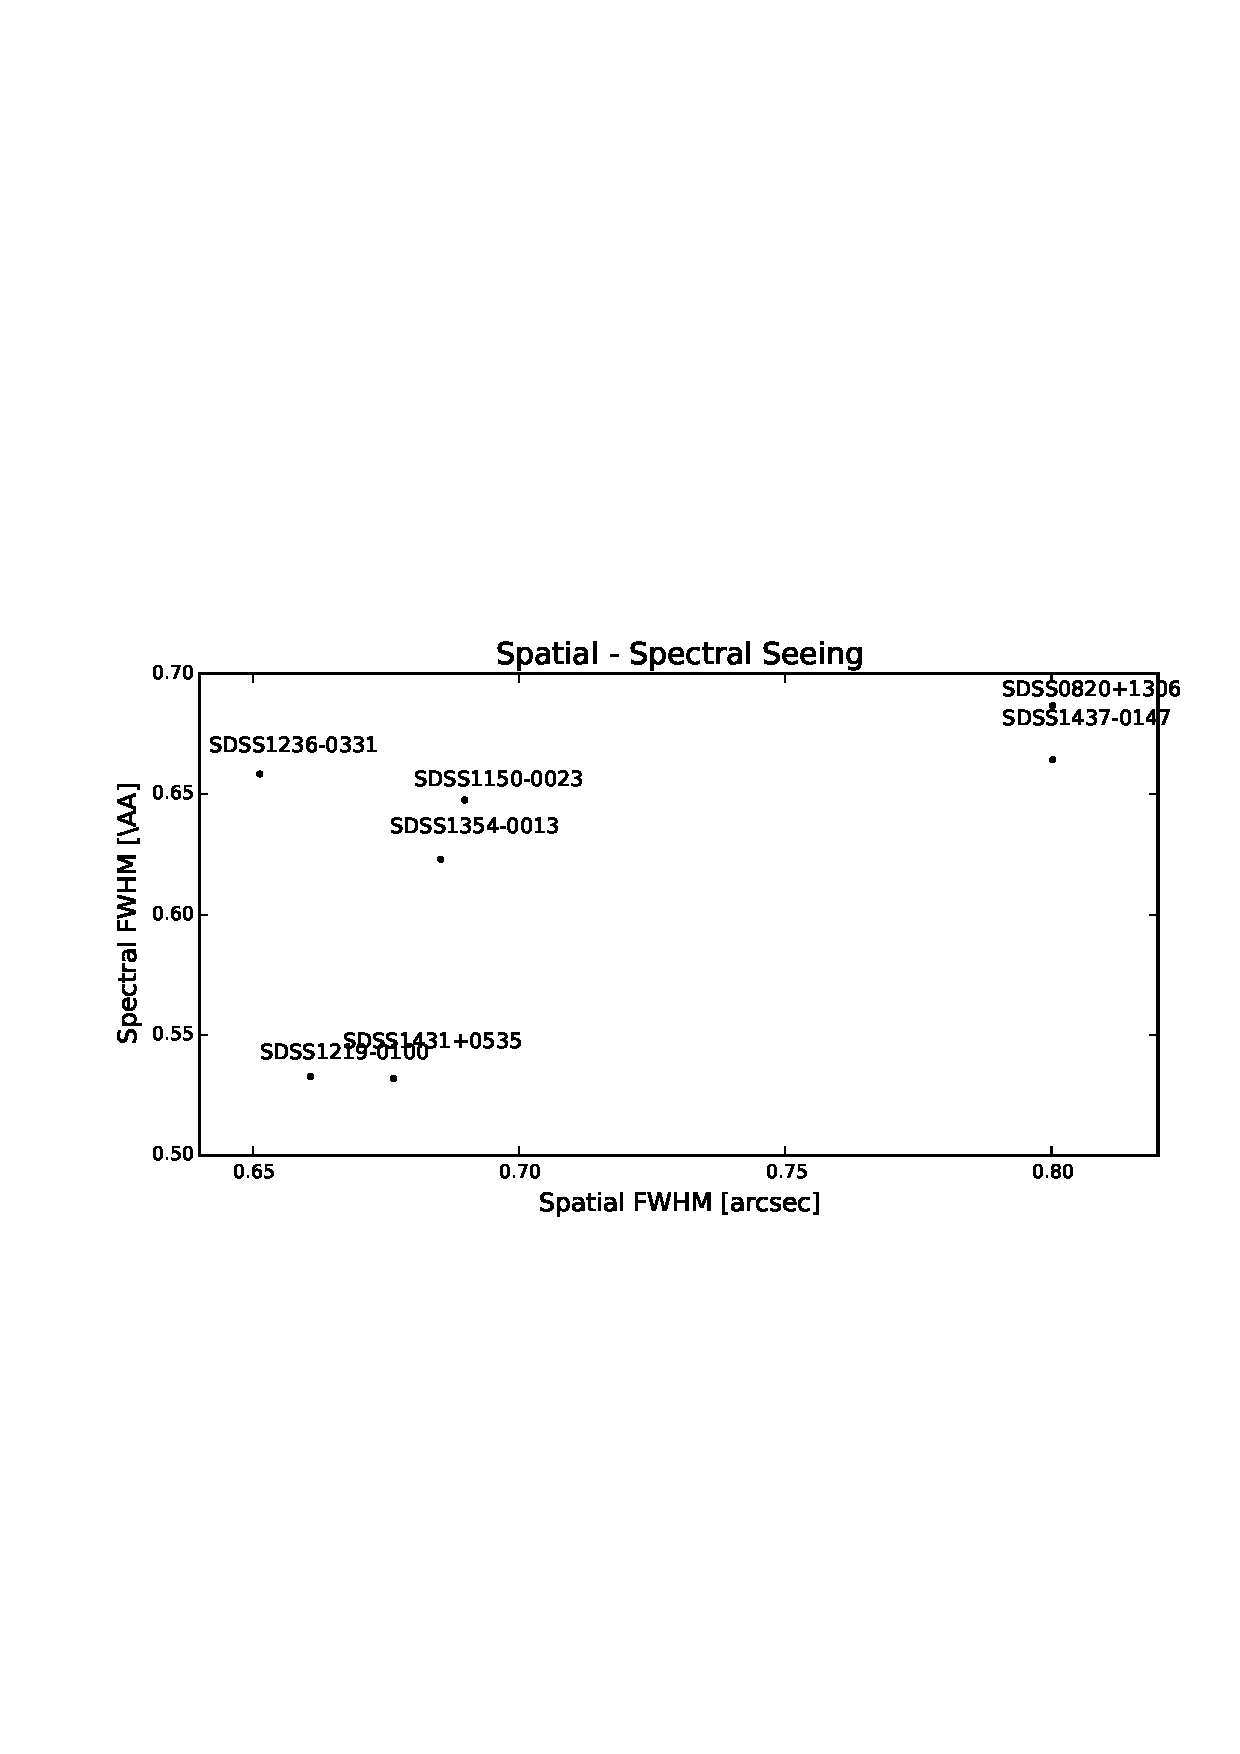
\includegraphics[width=0.99\columnwidth]{Figs/Seeing.pdf}
  \caption[]{Measured spatial seeing from the width of trace against the effective spectral resolution. All the observations are seeing-limited and thus the effective resolution will be higher than tabulated. (see text).}
\figlabel{seeing}
\end{figure}
%===========================================================================



As can be seen from \fig{seeing}, our observations are executed under excellent seeing conditions with corresponding resolutions between 11000 and 14500 in the visual arm with an average R$_{VIS}$ = 12750 - a factor of 1.7 increase compared the nominal resolution. 

%If we assume that the ratio of measured spatial FWHM to spectral FWHM measured in the visual arm remains constant we get the resolution in UVB and VIS from the width of the traces in the respective arms taking into account the different pixel-scale in the NIR arm. The real resolution is measured in the VIS data, and the improved resolution is then extrapolated to the UVB and NIR arms taking into account the different pixel scale in the NIR arm. 
%\qtodo{Johannes, the X-shooter Messiah, says this is fishy! You should definitely check up on this!}
%The spectral resolution is the spatial resolution convolved with the diffraction resolution (intrinsic spectral resolution). For very narrow intrinsic resolutions the corresponding Gaussian can be approximated by a Delta function. A Gaussian convolved with a delta-function leaves the gaussian unchanged. If this is the case, then the assumption I do is correct. 
%
%\begin{eqnarray}
%f_{spectral} = f_{spatial} \ast f_{grating}
%\end{eqnarray}
%
%If $f_{grating}$ is delta and this is the whole story, then what we do is correct. This could easily be checked by actually calculating the spectral resolution in the NIR arm.  
%
%
%We find the average resolutions for the observations: R$_{UVB}$ = 5150, R$_{VIS}$ = 12750, R$_{NIR}$= 8350. The resolution is important for the construction of the composite since we need to rebin the spectra to a common dispersion at a common redshift keeping the sampling of the pixels at the optimal Nyquist sampling (2 pixels per FWHM). 
%
%In pixel values we find a different spectral FWHM than spatial FWHM. These values should in principle be the same, but because X-shooter is an eschelle spectrograph, the seeing FWHM

The data were reduced using the ESO/X-shooter pipeline v2.5.2\citep{Modigliani2010} using the Reflex interface\citep{Freudling2013}. The spectra have been rectified on a grid with 0.2 \AA/pixel in the UVB and VIS arm and 0.6 \AA/pixel in the NIR arm, thus slightly oversampling even the highest-resolution spectra while minimizing the correlation between adjacent pixels in the rectification. The spectra were extracted by simple integration in the nodding window of the rectified image and were flux calibrated using photometric standards\citep{Vernet2010, Hamuy1994}. The seeing of the flux star observations were also significantly below the 5 arcsec slit width used for the observations of the spectrophotometric standard stars and slit losses will therefore be negligible. To check the accuracy of the flux calibration the corresponding spectra observed by SDSS\citep{Ahn2014} are compared to the X-shooter observations. Slight variations in individual spectra are detected in both flux level and apparent slope on the $\lesssim$10~percent level. This can both be attributed to erroneous flux calibration in one of the spectra or intrinsic object variability, which is observed to be of this order\citep{MacLeod2012, Morganson2014}. We discuss this in more detain in \sect{systematics}.
Telluric observations of hot B-type dwarf stars were taken close in time to allow for an accurate telluric correction which depends heavily on the atmospheric conditions at the time.



\begin{table*}
\centering
\begin{center}
\caption{Quasars in the composite. \label{tab:targets}}
% Trigger: 06:47
%\vspace{-0.3cm}
\begin{tabular}{cccccc}
\hline
\noalign{\smallskip}
SDSS identifier & $\alpha$(J2000) & $\delta$(J2000) & r &  $z_{SDSS}$ $^{(a)}$  &  $z_{fit}$ $^{(b)}$ \\  
\hline

%SDSS0043+0114  & 00:43:15.08 & $+$01:14:45.56 & 17.58 & 1.564      \\
%SDSS0155-1023  & 01:55:04.73 & $-$10:23:28.38 & 17.35 & 1.549        \\
%SDSS0209-0947  & 02:09:51.08 & $-$09:47:27.34 & 17.90 & 1.568       \\
%SDSS0303+0027  & 03:03:42.78 & $+$00:27:00.50 & 17.84 & 1.647       \\
%SDSS0323-0029  & 03:23:49.53 & $-$00:29:49.88 & 17.81 & 1.628      \\
SDSS0820+1306  & 08 20 45.39 & $+$13 06 18.99 & 15.91 & 1.1257 $\pm$ 0.0001 & 1.1242 $\pm$ 0.0001        \\
%SDSS0842+0151  & 08:42:40.63 & $+$01:51:34.14 & 17.62 & 1.485       \\
%SDSS1002+0331  & 10:02:48.15 & $+$03:31:55.98 & 17.74 & 1.482      \\
SDSS1150-0023  & 11 50 43.88 & $-$00 23 54.07 & 17.00 & 1.9804 $\pm$ 0.0002 & 1.9799 $\pm$ 0.00002       \\
%SDSS1158-0322   & 11:58:41.37 & $-$03:22:39.93 & 17.56 & 1.576        \\
SDSS1219-0100  & 12 19 40.37& $-$01 00 07.49& 16.82 & 1.5770 $\pm$ 0.0002  & 1.5831 $\pm$ 0.0003       \\
SDSS1236-0331  & 12 36 02.34 & $-$03 31 29.94 & 16.91 & 1.8239 $\pm$ 0.0002   & 1.8464 $\pm$ 0.0006        \\
SDSS1354-0013  & 13 54 25.24 & $-$00 13 58.06 & 16.68 & 1.5124 $\pm$ 0.0002 & 1.51237 $\pm$  0.00009         \\
SDSS1431+0535  & 14 31 48.09 & $+$05 35 58.10 & 16.74 & 2.0964 $\pm$ 0.0002 & 2.09985 $\pm$  0.00004     \\
SDSS1437-0147  & 14 37 48.29 & $-$01 47 10.79 & 15.44 & 1.3091 $\pm$ 0.0001& 1.30901 $\pm$  0.00002        \\

\hline
\hline
\end{tabular}
\end{center}
\noindent{

$^{(a)}$ Taken from SDSS .
$^{(b)}$ The fit method is described in the text. 
}


\end{table*}



 \tablabel{targs}



%====================================================================
\subsection{Telluric Correction}   \sectlabel{telluric}
%====================================================================

All ground based observations suffer from atmospheric absorption. This is especially true in the Visual (VIS) and Near-Infra-Red (NIR) arm of X-shooter where there are regions of telluric absorption with almost zero transmission from water vapor and other molecules. Because of the limited sample-size, it is desirable to avoid simply masking out regions of atmospheric absorption, but rather correct for it. To this end a method based loosely on the method employed in \citet{Chen2014} is developed.
To correct for the absorption an exact measure of the transmission of the atmosphere at the time of the observation is needed. The amount of absorption is heavily dependent on the exact conditions through the atmosphere and these changes on very short timescales. Observations close in time of a featureless telluric standard star is done for all observations and it is these observation that are used for the generation of the atmospheric transmission spectrum. 

%===========================================================================
\begin{figure}[t!]
  \centering
  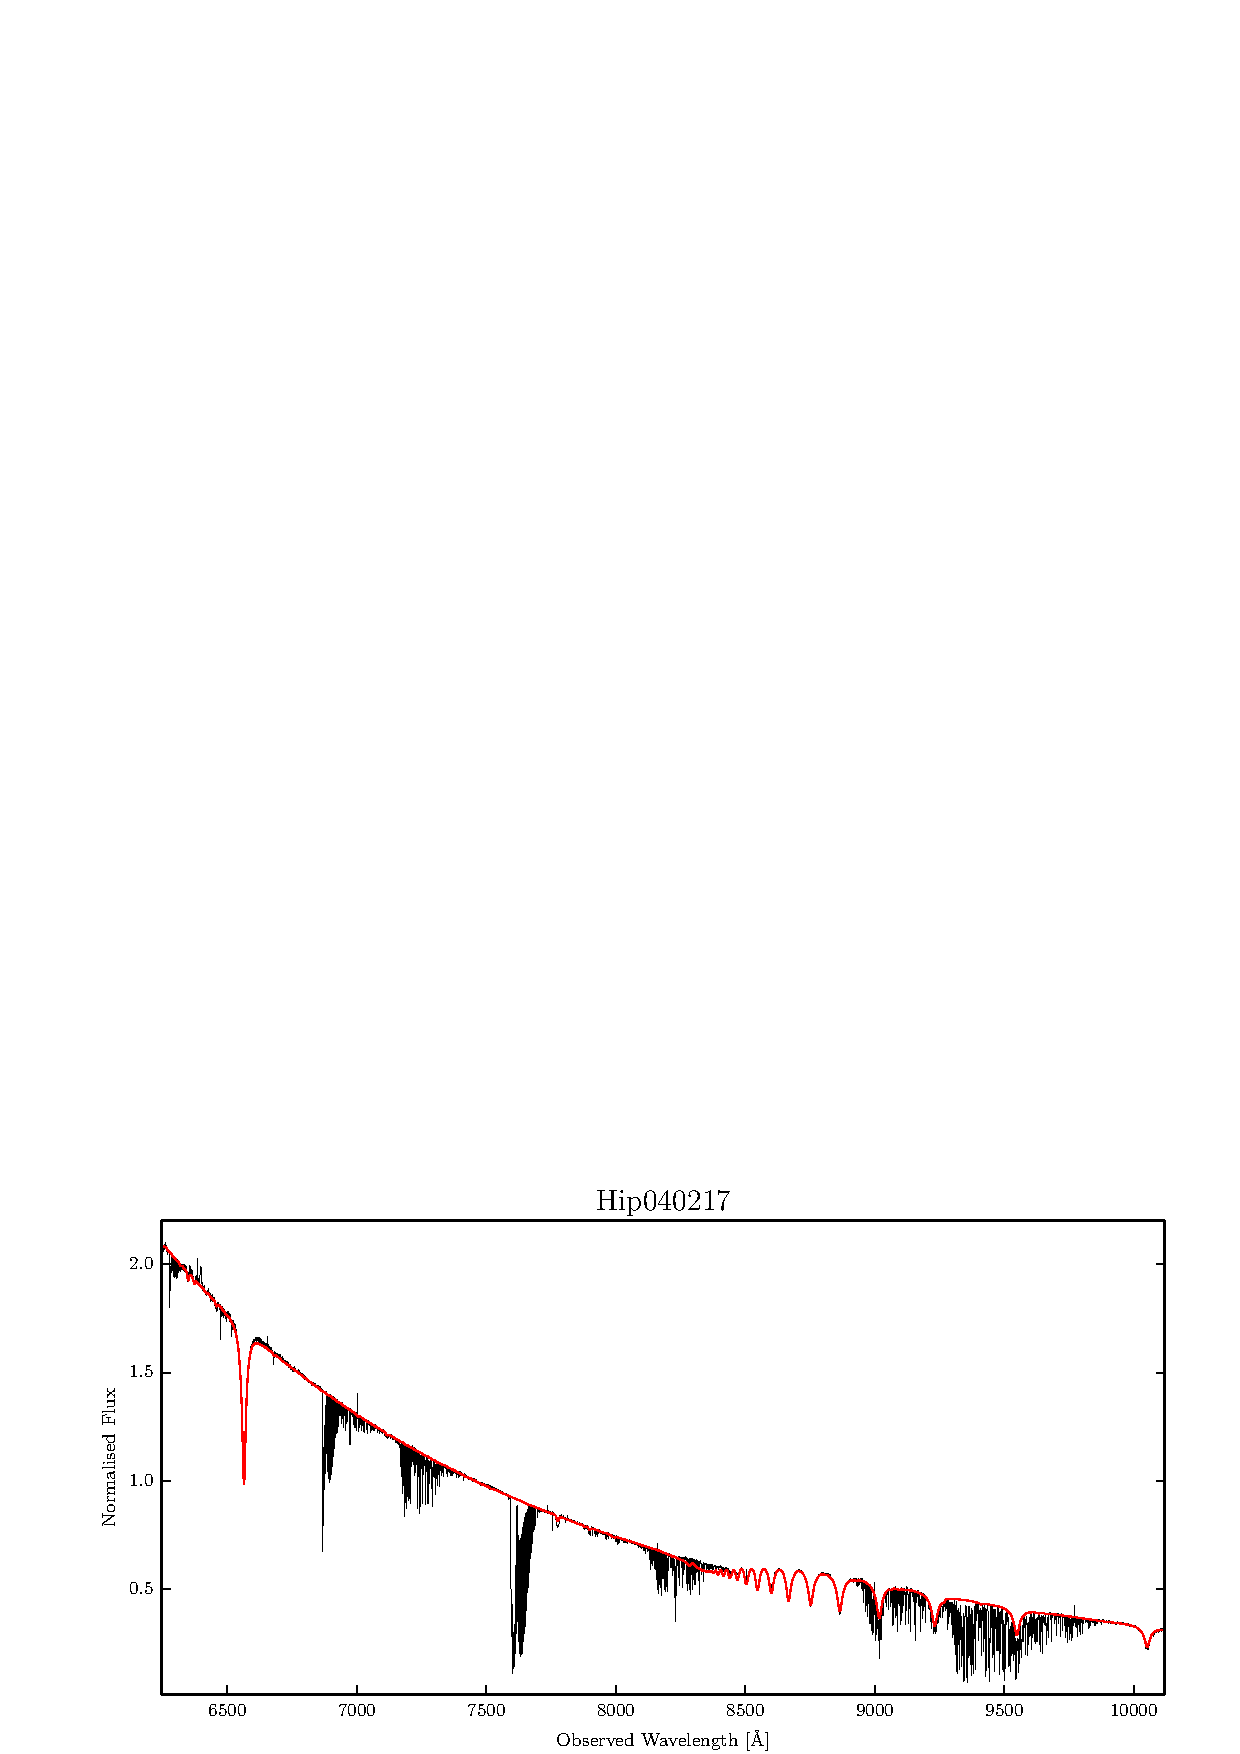
\includegraphics[width=0.99\columnwidth]{figs/tell_corr_QC.pdf}
  \caption[]{Telluric correction for quasar SDSS1431+0535 where brown is the uncorrected spectrum and purple is the corrected and teal is the corrected smoothed by 50 pixels. The regions of pure noise is where the atmospheric transmission is $\sim$ zero, thus only leaving noise after correction. Residuals after correction is visible, but noise image is corrected correspondingly and therefore giving less weight to regions severely affected for the weighted combination.}
\figlabel{telluric_qc}
\end{figure}
%===========================================================================


From the observations of the telluric standard star it is possible to calculate the atmospheric transmission spectrum by modeling the intrinsic stellar spectrum. The transmission spectrum is the fractional difference between the model and the observed spectrum. We model the telluric standard by finding the optimal linear combination of templates among the model atmospheres of G\"ottingen Spectral Library\citep{Husser2013}. Here the PHOENIX model stellar atmosphere code is used to create a grid of synthetic spectra in terms of effective temperature, metallicity and alpha element enhancement. To find the optimal template we simultaneusly fit for the instrumental profile broadening, velocity shift and optimal template using the penalized-pixel fitting software pPXF\citep{Cappellari2004} to find the linear combination of spectra and spectral broadening that minimizes $\chi ^2$ between our object spectrum and the found template . For the fitting we exclude all regions of strong telluric absorption since we only want to trace the continuum. After a transmission spectrum has been constructed from the telluric standard observations, the object observation closest in time is divided by the transmission, thus correcting the the absorption. 

 As can be seen in \fig{telluric_qc}, the intrinsic object spectrum is recovered relatively well. The regions where the continuum of the telluric standard is not found accurately will produce an erroneous transmission correction and introduce an error in the resulting corrected spectrum. We review the consequences of this in \sect{systematics}. 



%%%%%%%%%%%%%%%%%%%%%%%%%%%%%%%%%%%%%%%%%%%%%%%%%%%%%%%%%%%%%%%%%%%%%%%%%%%%
\section{Composite Construction}   \sectlabel{construct}
%%%%%%%%%%%%%%%%%%%%%%%%%%%%%%%%%%%%%%%%%%%%%%%%%%%%%%%%%%%%%%%%%%%%%%%%%%%%

There is not a unique way to construct a composite and the final result is influenced by the method employed. In the following we describe how the composite is constructed.

%====================================================================
\subsection{Determining the redshift}  \sectlabel{redshifts}
%====================================================================

Of crucial importance is determining the distance to the quasars to accurately move the objects to the rest frame. Getting the systemic redshift of quasars from emission lines is complicated by the complex physical structure of the broad line regions in which the broad emission lines are emitted. For the bright quasars selected for our composite many of the prominent high-ionization lines visible will arise in hot clouds with large peculiar velocities and will therefore be affected by systematic line-shifts\citep{Richards2002b}. To get a redshift closer to the systemic we choose \oiii$\lambda5007$,  arising in the narrow-line region and therefore less affected by systematic offsets{\color{red} Reference needed}. \oiii~is situated on a broad Fe-complex and slightly blended with \oiii$\lambda$4959 and \hb, with \hb~ both containing broad and narrow components. 
To get an accurate estimate of the redshift we mark both sides of the line belonging to \oiii$\lambda$5007 where it starts to become blended, fit a low order polynomial to the edges and subtract the estimated pseudo-continuum. We define a Gaussian in terms of the rest wavelength of \oiii~ and leave the redshift as a free parameter and then fit to selected region where a weighted minimization of the residuals is done using least squares and the confidence intervals on the best-fit parameters is determined by resampling from a multivariate Gaussian with best-fit values as the mean and a covariance matrix which is the estimated Hessian at the minimum. The weights used are the inverse variance, $ w =  \frac{1}{\sigma^2}$, where $\sigma$ is the statistical error of the spectrum. The 1$\sigma$ confidence intervals on the fit parameters are set by the 16th and 84th percentile of the resampling realizations. The formal errors obtained from the fit are bound to be under-estimating the true error, since correlation between the pixels are not taken into account. Least squares minimization do not guarantee to find the global minimum of the residuals, but we check visually that the fit is satisfactory. \oiii$\lambda$5007 is visible in all of our spectra in varying strength so additional refinement is not needed. As a starting guess for the redshift we use redshifts queried from SDSS and all fits are visually inspected to check if the fitted redshift is an improvement on the position of \oiii$\lambda$5007. We show a\oiii~fit in \fig{linefit}, where \hb, \oiii$\lambda$4959 and \oiii$\lambda$5007 are clearly detected and marked on the plot. Several broad underlying features make it difficult to model the entire complex by the three lines alone and therefore only the narrowest component of the \oiii-line is used for the fit. Additionally only the upper part of the total line flux is used in the fit. This is similar to what is done in \citet{VandenBerk2001}. A clear velocity offset is visible between the rest-frame determined by \oiii~and \hb. We take this as an indication of high peculiar velocities in the region of \hb-emitting clouds\qtodo{Is this right?}. We convert all vacuum wavelengths to air and transform all redshifts to barycentric standard-of-rest for consistent comparison with SDSS. For all of our spectra we find slight corrections to the SDSS redshifts, based on the fit to \oiii, as is also shown in \tab{targs}. We note that only two out of seven redshifts agree within the errors, but stress that the measured redshifts are not measured in a consistent manner and therefore offsets are expected. SDSS spectral redshift determinations are based on restframe UV lines which are known to exhibit substantial velocity shifts relative to the systemic redshift\qtodo{True? - Reference needed}.
%===========================================================================
\begin{figure}[t!]
  \centering
  \includegraphics[width=0.99\columnwidth]{Figs/LineFit.pdf}
  \caption[]{Gaussian fit of [OIII] $\lambda$5007. The red solid line is the linear-least-squared best fit with 1$\sigma$ confidence interval. Green dashed lines indicate the position of neighboring lines at the redshift of [OIII]. It can be seen that H$\beta$ is red-shifted as compared with the redshift of [OIII], indicative of large peculiar velocities.}
  \figlabel{linefit}
\end{figure}
%===========================================================================

%====================================================================
\subsection{Resampling} \sectlabel{rebin}
%====================================================================

Before combination of the spectra can be done, the spectra are moved to the local frame. Because of the varying redshifts of the objects, the spectra will have their spectral arms of X-shooter overlap at different wavelengths and thusly will have varyings sampling sizes. X-shooter, being a cross-dispersion echelle spectrograph, have a non-linear dispersion solution and in order to conserve the most information without oversampling, we need to choose a representative bin size on which to interpolate our spectra. The largest sampling is in the NIR arm and is $0.6$ \AA/pix with an average redshift of $z_{avg} = 1.6$ gives us the conservative bin size of $0.4$ \AA/pix in the rest-frame. Since our spectra have significantly better resolution than the nominal values and the UVB and VIS arms have a sampling of $0.2$ \AA/pix we will be discarding spectral information to make sure that we are not oversampling. We create a wavelength grid from 1000-11665 \AA~in steps of 0.4 \AA, giving $\sim$ 16000 spectral elements on which we interpolate the spectra. The input spectra are moved to the rest-frame by dividing the wavelengths with $(1 + z)$ and to conserve flux we multiply the flux density with a corresponding $(1 + z)$. The spectrum is then interpolated using a linear spline. The interpolated spectrum is resampled onto the newly defined common wavelength grid. Since the constituent spectra have different sampling than the target grid, we will introduce additional correlations between neighboring pixels. This is not taken into account in the reported statistical error of each spectrum which means we will be underestimating the errors. 

%====================================================================
\subsection{Extinction} \sectlabel{extinct}
%====================================================================

The spectra are all corrected for galactic extinction. Extinction values are queried from the reddening maps of \citet{Schlegel1998} using the recalibration from \citet{Schlafly2011}. Extinction values in a 2-degree radius around the source is extracted from the map and a arithmetic mean is used for the average value. The reddening law by \citet{Fitzpatrick1999} with optical total-to-selective extinction ratio $R_v = 3.1$ is used to deredden each spectrum. The average value of the reddening for our objects is small, $E(B-V) = 0.034$, so we expect any residual effect of the galactic extinction to be minimal. 


%====================================================================
\subsection{IGM absorption correction} \sectlabel{igm}
%====================================================================

At redshifts higher than $\sim1.6$, the rest-frame coverage of X-shooter goes bluewards of \lya~and are therefore heavily affected by \lya-forest absorption, blueward of the \lya-line. A normal way to correct for this absorption is to obtain a spectrum at a sufficiently high resolution to be able to trace the continuum emission by visual inspection. At $z < 2 $ the \lya~forest absorption is not yet heavily blended\qtodo{Reference needed}, and the X-shooter resolution allows us to effectively trace the continuum. To recover the continuum we insert evenly spaced points every 50 pixels, blueward of \lya, each point calculated from the median value of the constituent pixel values. This procedure equals binning the spectrum by 50 pixels and using the median value. We then manually delete points that are not sufficiently smoothly varying, signifying points affected by \lya-forest absorption. When the points represents the visually estimated continuum, a linear spline is the used to interpolate between the points onto the sampling of the original wavelength array. We then concatenate this new continuum estimate with the original spectrum, at \lya. The objects SDSS1150-0023, SDSS1236-0331 and SDSS1431+0535 are the ones contributing the compostite at these wavelengths. \qtodo{References to support this?}



%====================================================================
\subsection{Normalisation}  \sectlabel{norm}
%====================================================================

In order to combine the spectra in a meaningful way, we need to normalize the spectra as not to favor one spectrum over the other and biasing our final spectrum towards a certain kind of shape since the aim is to find a representative continuum shape of the composite. Depending on the type of features we are interested in and on the combination method employed, there are different ways to achieve this normalization. Because the spectra have different absolute flux-scales, a popular way to normalize is to order the spectra in increasing wavelength, starting with the lowest redshift, and scale the entire spectrum by the median value of the flux and in the overlapping region with the next spectrum, combining the spectra consecutively, always scaling to overlapping region. The region chosen and the order of combination will affect how the final spectrum will look\citep{Francis1991,Brotherton2000,VandenBerk2001,Glikman2006}.
In principle the variance of the composite should reflect the intrinsic variability of constituent spectra, but the region to which we scale will affect the absolute scale of the variance. To make the variance reflect the intra-spectral variability the most, the spectra have been scaled in the region with the least intrinsic continuum variability, which decreases with wavelength, at least up to 6000 \AA \citep{VandenBerk2004}. The region closest to 6000 \AA~free of contaminating emission is just redwards of H$\alpha$ in the region 7000- 7500 \AA. Each spectrum have been divided by the median flux in this region, thus the normalization is independent and the order in which the combination is done does not matter. 
Before any combination is done, all spectra have been run through a filter, where if the change from pixel to pixel is greater than 20 \%, the pixel is flagged and excluded from the combination. This is to exclude noisy pixels and pixels affected too seriously by telluric absorption correction. We have investigated whether this exclusion changes the shape of the combined continuum and no effect was visible. This way of flagging noisy pixels, ensures that we retain as much signal as possible without introducing very noisy isolated pixels. As many as 5 percent of the total number of pixels is rejected in the worst case. 

%====================================================================
\subsection{Combination}  \sectlabel{combine}
%====================================================================

Choosing the right combination method is tricky business and different method can yield slightly varying results. The first assumption is that at each pixel, the constituent spectra have a Gaussian distribution around a sample mean and that this mean reflects the expectation value of the sample. Since we have a relatively small sample, even investigating whether we are sampling from a Gaussian distribution is ambiguous. To make a test for normality, we take the mean of 100 pixels along the composite, assuming that the continuum is flat, and make a quantile-quantile plot. Given that we are sampling from a normal distribution the blue points should fall on the red line. Since we one have 7 pixels, determining whether the constituent spectra are normally distributed, is a guess at best. We show the Q-Q plot in \fig{normality}, where it is not immediately evident if we are sampling from a normal distribution, but it is not a bad guess. We run a Shapiro-Wilk test where the same 100 pixels from the central part of the spectrum is used. On each individual collection of pixels we test gives us a 2-sided chi squared probability for the hypothesis test, under the null hypothesis that the sample comes from a normal distribution. With an average over the pixels of $p = 0.37$ we can a least not reject, that we are sampling from a normal distribution. Since we have no reason to expect that we are sampling from a Gaussian distribution and that the distribution is expected to change with wavelength increasing in width as the distance to the normalization region increases, a certain caution is warranted. 

%===========================================================================
\begin{figure}[t!]
  \centering
  \includegraphics[width=0.99\columnwidth]{Figs/normality.pdf}
  \caption[]{Quantile-Quantile plot as a test for normality. An average over 100 pixels in the central regions where the continuum is assumed to be relatively flat is used. The inverse cumulative distribution for the sample is constructed and the plotted against the corresponding quantiles for a normal distribution. The 45 degree line is if we are sampling for a normal distribution. Since the points are slightly steeper, this indicates a more dispersed distribution.}
 \figlabel{normality}
\end{figure}
%===========================================================================

In the case for uncorrelated pixels the minimal variance point estimation for the sample mean is the inverse variance weighted mean, given again that the constituent spectra at each wavelength bin can be treated as a stochastic variables that follow a normal distribution $\mathcal{N}(\mu, \sigma_i^2)$ with mean $\mu$ and variance $\sigma_i^2$. The inverse variance weighted mean is calculated as:

\begin{eqnarray} \eqlabel{wmean}
\bar{f_{\lambda}} &=& \frac{ \sum_{i=1}^n \left( f_{\lambda, i} \sigma_{\lambda, i}^{-2} \right)}{\sum_{i=1}^n \sigma_{\lambda, i}^{-2}},
\end{eqnarray}

with the variance of the weighted mean given as: 
 
\begin{eqnarray} \eqlabel{sigma-wmean}
\sigma_{\bar{f_{\lambda}}}^2 &=& \frac{ 1 }{\sum_{i=1}^n \sigma_{\lambda, i}^{-2}}.
\end{eqnarray}

Because X-shooter is cross-dispersed it is necessary to resample the image on a rectified image and this process introduces correlations between adjacent pixels. Since we have again rebinned the pixels to the common pixel scale additional correlation between adjacent pixels will be introduced both the the flux spectrum and in the error spectrum, meaning that we will be underestimating the errors in the resulting composite spectrum where the statistical noise will be hiding in pixel-top-pixel variations. Additionally, since our objects are fairly bright, the Poisson noise in our spectra will be non-negligible and thus we are incorporating the pixels values themselves intro their weight which leads to a bias in the result towards spectra of lower signal-to-noise. We check how the combination method employed affects the qualitative features in our spectrum in \sect{systematics}.

%====================================================================
\subsection{Absolute magnitudes} \sectlabel{absmag}
%====================================================================

In order to make a meaningful comparison with other composites and to the parent population of quasars, synthetic apparent magnitudes are calculated and then, using the redshift, converted to absolute magnitudes. Synthetic photometry is the process by which the apparent magnitudes in a bandpass is obtained from a spectrum by convolution with the filter quantum efficiency curve \cite{Bessell2005}. Following \citep{Bessell2012, Casagrande2014} we calculate the synthetic AB magnitudes using:

\begin{eqnarray}\eqlabel{abmag}
m_{\textmd{AB}_x} &=& -2.5  \frac{\int f_\lambda \,  T_{x}  \, \lambda \,  d\lambda} 
{\int  T_{x} \,  (c / \lambda) \,  d\lambda}  - 48.60,
\end{eqnarray}
 
 
where $f_\lambda (\lambda)$ is the observed flux in units of \fluxunit~ for the spectra shifted to rest(z=0) and $T_{x} $ is the total system fractional throughput in band $x$. The apparent magnitude can then be converted to absolute magnitude using:

\begin{eqnarray}\eqlabel{absmag}
M_{\textmd{AB}_x} &=& -5 \log_{10} \left[  \frac{D_L }{10 \mathrm{pc}}   \right] + m_{\textmd{AB}_x} ,
\end{eqnarray}
with the \textit{luminosity distance}, $D_L$,  obtained using a standard cosmological calculator\footnote{astropy.cosmology}.
 The largest compilation of quasar absolute magnitudes to date is \cite{Shen2011}, in which $\mathrm{M_i (z=2)}$ for the 105,783 quasars in DR7 is presented. To get the corresponding magnitudes for the composite constituent quasars at $z = 2$, the wavelengths are shifted and the flux scaled correspondingly to conserve flux. Using the SDSS i-band filter transmission curve\footnote{\url{http://classic.sdss.org/dr7/instruments/imager/filters/i.dat}} interpolated to the shifted wavelength together with \eq{abmag} and \eq{absmag} yields the desired quantities. The results are shown in \tab{targs} and comparison is done in \sect{parents}
 It is also possible to calculate the magnitude correction from $z = 0$ to $z = 2$ following \cite{Richards2006a} Equation (1), in which a pure power law is assumed for the quasar composite. For the i-band, this procedure consistently underestimates the magnitude of the correction, due to the bandpass being shifted to a region with heavy line emission, with a mean underestimation of $0.35 \pm 0.14$ mag, where the uncertainty is the 1-$\sigma$ error.







%%%%%%%%%%%%%%%%%%%%%%%%%%%%%%%%%%%%%%%%%%%%%%%%%%%%%%%%%%%%%%%%%%%%%%%%%%%%
\section{Results}   \sectlabel{results}
%%%%%%%%%%%%%%%%%%%%%%%%%%%%%%%%%%%%%%%%%%%%%%%%%%%%%%%%%%%%%%%%%%%%%%%%%%%%


We show the weighted mean composite in \fig{combined}. Characteristic features of quasars are readily visible. We see several prominent emission lines across the entire spectral range which includes both very broad high-ionization lines and narrower low-ionization lines as is typical for quasar spectra, with both broad and narrow lines superposed with multiple components\citep{Baldwin1995}. We have marked the position and name of the most prominent lines and overplotted them in \fig{composite}.  Analysis of the lines are beyond the scope of this paper.

 %===========================================================================
 \begin{figure*}[t!]
   \centering
   \includegraphics[width=2.0\columnwidth]{Figs/Combined.pdf}
   \caption[]{\textit{Top panel:} Composite spectrum with prominent emission lines marked. \textit{Upper middle panel:} Measure of intra-spectrum variability. The standard deviation of the constituent spectra as a function of wavelength. To normalize for differing slopes in between the different spectra, the fitted slope in each of the constituent spectra is divided by the standard deviation. 
   \textit{Lower middle panel:} Signal-to-noise. The composite spectrum is divided by the error spectrum, thus directly giving a measure of the signal strength.
   \textit{Bottom panel:} Number of contributing spectra as a function of wavelength, 
   
   }
  \figlabel{combined}
 \end{figure*}
 %===========================================================================


As is often seen\citep{Elvis2001}, the continuum level is shrouded by a myriad of emission lines, balmer continuum and Fe-complexes scattered across the entire spectrum, making the intrinsic shape of the continuum difficult to estimate. In \fig{composite}, we plot the composite spectrum on a log-log scale on which a power-law appears as a straight line and a linear trend is visible. 

The composite spectrum covers from \lyb ~in the bluest part of our spectrum to Pa$\gamma$ in the reddest, where a stright line adequately describes the continuum from \lya~and redwards. Bluewards of \lya~the spectrum is affected by \lya-forest absorption and the spectral continuum changes slope. The change in slope is a consequence of the accretion disk mechanism responsible for the continuum which generates a continuum with a spectral break which position is set by the temperature of the disk\citep{Pereyra2006}. The correction for \lya-forest absorption is described in \sect{igm}.


 Between $\sim2000$ \AA~ and $\sim5000$ \AA, excess emission compared with a pure power is detected, consistent with  the \textit{small blue bump} \citep{Wills1985}, which consists of a blend of balmer continuum and \feii ~lines, both broad and narrow.

 A single quasar spectrum is usually modeled by a power-law, $f_{\lambda} \propto \lambda^\alpha$, but a weighted mean spectrum of a sample of power-laws does not, in general, result in a power-law with the slope mean of the individual spectra. In principle a geometric mean of a sample of power-laws should result in a power-law with index being the mean index, as is shown in \sect{math}. We compare the composite obtained by taking the geometric mean with that obtained by the weighted average and no significant difference is detected between the two composites. We therefore take the  weighted mean composite as representative of the constituent spectra. This potential cause of systematic error due to combination methods is investigated more in \sect{systematics}.

%1300 - 1350, 1425 - 1475, 5500 - 5800, 7300 - 7500
%1350 - 1365, 4200 - 4230, 5500 - 6035, 7800 - 7950
Regions free of contaminating emission are very scarce and fitting a power-law to the composite in manually specified regions is not guaranteed to reflect the spectral index of the continuum. A quantitative measure of the shape can be obtained by carefully selecting regions that appear relatively unaffected by emission in excess of the continuum. The regions that cover the widest wavelength range are: 1300 - 1350, 1425 - 1475, 5500 - 5800, 7300 - 7500\AA, which we use to fit both with a single power-law and a broken one, with the break redwards of \hb~at 5700 \AA~as is reported by other authors\citep{VandenBerk2001}. For the single power law we obtain $\alpha_\lambda = -1.70$, where for a broken power law we obtain a spectral index; $\alpha_\lambda = -1.70$ below 5700 \AA, and $\alpha_\lambda = -1.72$ above, consistent with a single power law describing the continuum from  \lya ~to Pa$\gamma$. The break in \cite{VandenBerk2001} is attributed to contamination from the host galaxies\citep{Glikman2006} and adapting the same interpretation, gives support to the assumption about the negligible host galaxy contribution present in the composite presented here. A detailed comparison with existing composites in \sect{comparison}.


%====================================================================
\subsection{Applicability of the composite}  \sectlabel{application}
%====================================================================


To test the applicability of the composite, it is used to determine the dust content of a sample of three red quasars taken from the HAQ (High A$_V$ QSO) survey\qtodo{Direct reference?}. The HAQ survey consists of quasars selected on the basis of their optical colors in SDSS and near-infrared in UKIDDS to identify the reddest and therefore most dust-extincted quasars which are missed by traditional color selection criteria. A complete description of the sample criteria and the data are presented in \citet{Fynbo2013} and \citet{Krogager2015}. The dust content can then be inferred by reddening the composite with an extinction law parameterized by \cite{Gordon2003} to match the object spectrum. The parametrization allows the redshift of the object quasar and the magnitude of visual extinction, A$_V$, to be found by minimizing the residuals between the object and the composite. A detailed description of the fitting method is given in \cite{Krogager2015}.

The three quasars have been selected to have varying amounts of extinction and have differing redshifts. We show the result for quasars HAQ2221+0145, HAQ1115+0333 and HAQ2231+0509 in \fig{application} where the success of matching the composite with quasars of very different shapes is visible. 

Following \cite{Wang2012}, the previous composite used to fit for the dust amount consists of the composite generated by \cite{VandenBerk2001} stitched together with the composite by \cite{Glikman2006} at 3000 \AA. Thus, two different composites built from differing samples have been treated as a single composite. That this has been successful is a testament to the similarity of quasars across a large range of apparent physical conditions. 
The values obtained with the newly generated composite is entirely consistent with the values published in \cite{Krogager2015}, which is encouraging for the previous use of stitched template. A detailed comparison between the different composites is done in \sect{comparison}.

%===========================================================================
\begin{figure}[t!]
 \centering
 \includegraphics[width=0.99\columnwidth]{Figs/application.pdf}
 \caption[]{The dust extinction, $A_V$, and redshift has been inferred for three HAQ quasars by fitting for the amount of reddening required to match the template with the observed spectrum. For varying amount of extinction at different redshifts, consistent results are found with previous usage of stitched composites.}
 \figlabel{application}
\end{figure}
%===========================================================================
 
 %%%%%%%%%%%%%%%%%%%%%%%%%%%%%%%%%%%%%%%%%%%%%%%%%%%%%%%%%%%%%%%%%%%%%%%%%%%%
 \subsection{Intra-spectrum variability}  \sectlabel{variability}
 %%%%%%%%%%%%%%%%%%%%%%%%%%%%%%%%%%%%%%%%%%%%%%%%%%%%%%%%%%%%%%%%%%%%%%%%%%%%
 
 To gauge the intra-spectrum variability, the standard deviation of the flux points at each wavelength divided by the composite reflects the fractional sample variability, where by construction this is minimized at the region chosen for normalization - in this case, just redwards of \ha. The general shape of the variability curve is therefore rather uninformative, but nonetheless valuable information can still be gained by inspection. We show the computed fractional variability in \fig{combined}. The sample variability contains both the temporal variability and the intrinsic population variability which is not possible to separate with single-epoch data and therefore potential conclusions should be wary of this degeneracy.
 Significant variation is visible in the the lines of \civ, \mgii, \oiii~ and lines of hydrogen as well as in the \feii-complexes centered around \hb. From 5800 - 11000 \AA~the continuum variability stays almost constant which could indicate a more stable continuum, both temporally and population-wide \qtodo{Is this pushing it too far?}. An increase in variability is observed redwards of 5800 \AA~due to slightly varying power law slopes of the constituent spectra. In the region bluewards of \lya~ the fractional variability reaches 60 percent, testament to the stochastic nature of the lyman alpha forest, but the reader is cautioned that only three spectra contribute significantly at these wavelengths.  
  
%===========================================================================
\begin{figure*}[t!]
\centering
\includegraphics[width=1.98\columnwidth]{figs/compo_full_sample.pdf}
\caption[]{X-shooter quasar weighted arithmetic composite on a linear wavelength scale. The position of several prominent emission lines are marked. Overplot is the corresponding composite generated from the full sample of SDSS quasars fulfilling the selection criteria and general agreement is observed, albeit with a brighter balmer continuum in the SDSS-constructed composite. In red and green is shown the results from fitting both a pure and a broken power-law to the regions specified in \sect{results} and they are observed to be consistent.}
\figlabel{composite}
\end{figure*}
%===========================================================================

%%%%%%%%%%%%%%%%%%%%%%%%%%%%%%%%%%%%%%%%%%%%%%%%%%%%%%%%%%%%%%%%%%%%%%%%%%%%
\section{Discussion}  \sectlabel{discuss}
%%%%%%%%%%%%%%%%%%%%%%%%%%%%%%%%%%%%%%%%%%%%%%%%%%%%%%%%%%%%%%%%%%%%%%%%%%%%

The applicability of quasar composites as tools for template matching and dust estimation largely hinges on the ability of the composite to represent an intrinsic target spectrum. The broad usage and success of previous composites largely confirms this ability. That the composites constructed are representative for a large group of differently selected quasars is a testament to the homogeneity of the quasar population and the universality of the emission mechanism.
The remarkable uniformity of the average spectral properties across luminosity and redshift indicate very similar underlying physical mechanisms which can be understood in terms of Eigenvector 1\citep{Boroson1992, Francis1992} where the Eddington ratio drives the relative strength of the lines and orientation effects influences the observed kinematics of the lines\citep{Shen2014a}. The specific local physical conditions which regulate the accretion rate then accounts for the majority of the inter-quasar variation. In this section we will investigate whether the targets selected are simply scaled-up version of average quasars, or remarkable in some sense.


%%We have to be careful with regards to the conclusions and the sample selection. We have selected bright quasars, but we can only say something about the mean of this particular sample and not something about the general population of quasars. If there exists an intrinsic population of quasars who are redder, this effect will be degenerate with dust, and fitting for the dust are not guaranteed to result in robust results. This is of major concern.  
%\qtodo{Talk to Jens about this again}.
%
%Something extremely profound.
%
%Due to the intrinsic brightness of our objects, we expect the black-hole mass to be high, compared lower-brightness objects. \citet{Lusso2015} section 5.5 find that the break in power-law slope at$ \sim 920$ \AA is which does not agree with Shakura sunyaev prediction. They need high black-hole spin or wrong black-hole masses to make the two models fit.  
%If a model SED for a quasar is needed a shallower slope than the one from \citep{VandenBerk2001}, is found, 
%\jstodo{Investigate this further}

%====================================================================
\subsection{Comparison to the parent population}  \sectlabel{parents}
%====================================================================

Figure 1 in \cite{Shen2011} presents the distribution of M$_i(z=2)$ as a function redshift for quasars spectroscopically confirmed from the SDSS. The black dots represents about half of the objects and are uniformly selected to $\sim$90 percent completeness\citep{Richards2002, VandenBerk2005}. It is clear that the sample presented here represents some of the brightest quasars existing between redshift 1 and 2. It is therefore potentially a biased subset of the parent quasar population. Quasars have previously been shown to exhibit a large degree of homogeneity over many orders of magnitude \citep{Dietrich2002}, but this is only true for quasars resembling \textit{average} quasars. To ensure that the targets selected for this sample are not outliers in color, the spectrophotometric colors are compared to those of the quasar population presented in \citet{Paris2014}\footnote{\url{https://www.sdss3.org/dr10/algorithms/qso_catalog.php}}. We show the comparison in \fig{color_comparison}. From the magnitudes we first confirm that the quasars selected here are among the intrinsically brightest visible in i-band with a 2.8 sigma magnitude distance from the mean absolute i-band magnitude at redshift 2, M$_i(z=2)$. Despite their luminosity their colors are representative for the subset fulfilling the selection criteria. In \sect{application}, the composite generated here was used to fit for the dust content of quasars with varying degree of extinction and consistent results were obtained as compared with composites generated from other subsamples of the parent population. For a comparison between SDSS and quasars detected in \textit{GALEX}, UKIDSS, \textit{WISE}, 2MASS and \textit{Spitzer}, see Figure 2 in \cite{Krawczyk2013}.


 %===========================================================================
 \begin{figure}[t!]
   \centering
   \includegraphics[width=0.99\columnwidth]{Figs/color_comparison2.pdf}
   \caption[]{Quasar color, g-i,  as a function of redshift, z. The full quasar sample from SDSS DR10 \citep{Paris2014} is shown in grey color. Bounding contours show the 0.5, 1, 1.5, 2 $\sigma$ contours of the density of points. The blue-grey points are individual quasars from the SDSS sample which satisfy $r <= 17$. Overplotted in blue are the quasars constibuting to the composite presented here. The quasar colors have been marginalized over in the right side where the tall blue lines are at the position of the composite quasars and the short blue-grey lines are from all quasars fulfilling the selection criteria.}
  \figlabel{color_comparison}
 \end{figure}
 %===========================================================================

Because of the high luminosity of the objects presented here, several differences in the properties are expected as compared to those of the parent quasar population. The physical scales locally are expected to be larger\citep{Bentz2013}, which will make variability timescales longer and variability magnitudes smaller\citep{VandenBerk2004}, see also \citet{Schmidt2012}. Black-hole masses as determined from \mgii~increases with luminosity\citep{wu2015} which in turn affects the temperature of the accretion disc\citep{shakura1973, Pereyra2006} and thereby the position of the "big blue bump" and the degree to which the continuum is well modeled by a single power-law\citep[see also][for a discussion]{Lusso2015}. As can be seen from \fig{color_comparison}, the quasars selected for the composite represents average colors for the subset fulfilling the sample cuts. An immediate consequence of this will be, that the amount of dust inferred using this composite will be an average content, because the object which is sought modeled, can have an intrinsic quasar continuum shape that is different from what is constructed here, \citep{Richards2003, Hopkins2004a}. A population of intrinsically redder quasars exists\citep{Glikman2012} and the uncertainty in the inferred amount of extinction is therefore larger in these types of surveys, also targeting the reddest quasars. 
Since the \textit{true} intrinsic dereddened quasar color distribution is likely broad with a range of slopes, a caveat of using this composite that the amount of extinction inferred will be the average amount over a large sample.



%====================================================================
\subsection{Comparison to the sample population}  \sectlabel{sample_pop}
%====================================================================



A further bias can, because of the low number statistics used for the sample presented, that the targets are not representative for the population fulfilling the cuts imposed in the selection. As highlighted in \fig{color_comparison}, the objects selected here are also bluer than full sample fulfilling the selection criteria. To quatify the bias against the selection, we construct a composite in an identical fashion consisting of all SDSS quasar fulfilling the selection criteria. 
In \fig{composite} we overplot the composite generated from the SDSS spectra of the full sample fulfilling the selection criteria on the one constructed with X-shooter. It is clear that there are small differences in the shape of the composite constructed from the full sample and the small sample, but qualitatively the shape remains the same. Calculating the slope in each individual SDSS spectrum yields $\alpha = -1.6\pm 0.3$, but this number is difficult to interpret due to the narrow continuum region free of emission lines(1300 - 1350 \AA~and 1425 - 1475 \AA). It is comforting nonetheless that they are consistent within the errors. We investigate the effect of this in \sect{systematics}.


%====================================================================
\subsection{Comparison to existing composites} \sectlabel{comparison}
%====================================================================

A comparison to existing composites is not straightforward due to the different selection criteria that have been employed in the construction and thus the different composites are not guaranteed to represent the same population - most likely they will not. We compare to composites from the literature by the following authors: \citet{VandenBerk2001, Lusso2015, Glikman2006, Telfer2002, Francis1991}. The composite by \citet{VandenBerk2001} consists of 2204 SDSS quasars at $z_{median} = 1.253$ with absolute M$_{r'}$-magnitudes between $-18.0$ and $-26.5$ and therefore intrinsically fainter and lower redshift objects. \cite{Lusso2015} used 53 quasars observed with WFC3 at $z \sim 2.4$ with absolute i-band magnitudes at redshift 2, M$_i(z=2) ~\sim -28.5$, so of comparable brightness, but slightly higher distances. For constructing the composite, \cite{Glikman2006}  used 27 objects at $z \sim 0.25$ with an average absolute i-band magnitude M$_i \sim -24$ observed with IRTF, therefore constituting a much fainter, much lower redshift sample. \cite{Lusso2015} calculated the M$_i(z=2)$ magnitudes for the 184 constituent objects in \cite{Telfer2002} observed with FOS, GHRS and STIS onboard HST and find an average M$_i(z=2) \sim -27.5$ at $z \sim 1.2$, which yields a composite of fainter, more nearby sources. Lastly \cite{Francis1991} generated a composite from  688 LBQS(Large Bright Quasar Survey)-quasars observed mainly with MMT(Multiple Mirror Telescope). The absolute magnitudes cover $\sim -22$ and $\sim -28$ at a redshift-range $0.05 < z  < 3.36$ subject to a significant Malmquist bias for which the mean absolute magnitude is a strong function of rest-frame wavelength, with the brightest objects contributing at shortest wavelengths and visa versa for the faint objects. 

Despite the variation across selections criteria, luminosities and redshifts, a remarkable similarity in the overall shape is visible over a large wavelength range. The simultaneous existence of lines arising in such different environments around objects differing many orders of magnitude in luminosity is because varying conditions in the emitting clouds ensure that each ionic species have optimal conditions to produce line emission\citep{Baldwin1995}.  Significant differences between the composites are visible redwards of \lya~where different methods for IGM absorption correction has been employed. No correction has been applied in the composites by \citet{Francis1991, VandenBerk2001} and a sharp decrease in continuum flux is detected. Because higher redshift objects contribute most a shorter wavelengths, significant \lya~alpha absorption is expected regardless due to the \lya~opacity evolution\qtodo{Refernce}. The IGM correction of \citet{Telfer2002} is a hybrid in which some manual and some statistical correction has been applied. \citet{Lusso2015} rely on a sophisticated, purely statistical correction which has been calculated by integrating the neutral hydrogen column density distribution at $z \sim 2.4$ measured by \cite{Prochaska2014b}. The IGM correction in X-shooter composite presented here is done in each individual spectrum where resolved lines are interpolated over. Good agreement is found with \cite{Telfer2002}, but underestimated as compared to \cite{Lusso2015}. As argued by \cite{Lusso2015}, an explanation for this discrepancy is the underestimation of the correction needed to account for unidentified Lyman limit absorbers. Due to the resolution of the instrument and at the redshifts probes, this should not be a significant effect on the sources observed here. 
Differences in the emission lines is also visible. This is to be expected due to the highly varying magnitudes of the constituent objects for the different composites where a decreasing equivalent line width is expected with increasing luminosity\citep{Baldwin1977}. 
Above 5000 \AA, a clear discrepancy is visible to the \cite{VandenBerk2001}-composite which may be due to host galaxy contamination\citep{Glikman2006}. From \cite{Shen2011}, Figure 9. it is confirmed that this effect is not affecting the X-shooter composite presented here, due to the extreme luminosities, which we investigate in \sect{systematics}.
 %===========================================================================
 \begin{figure*}[t!]
   \centering
   \includegraphics[width=1.99\columnwidth]{figs/composite_comparison.pdf}
   \caption[]{Comparison of different composites. The composites by \citet{Lusso2015, VandenBerk2001, Telfer2002, Francis1991} are normalized to the X-shooter composite at $\sim 1450$ \AA~and the composite by \citet{Glikman2006} is normalized to ours at $\sim 3850$ \AA. Significant differences is visible blueward of \lya~due to differing IGM correction methods. Above 5000 \AA~ significant host galaxy contamination is visible in the composite by \citet{VandenBerk2001}. Overplot in blue is a pure power law with slope $\alpha = -1.7$ and normalized at $\sim 1450$ \AA.}
  \figlabel{composite_comparison}
 \end{figure*}
 %===========================================================================
 \begin{table}
\centering
\begin{center}
\caption{Power law slopes from different combination methods. \label{tab:targets}}

\begin{tabular}{cc}
\hline
\noalign{\smallskip}
Reference &  FUV slope, $\alpha$$^{(a)}$ \\  
\hline


Selsing et al. 2015  & $-1.70$   \\
Lusso et al. 2015  & $-1.39$   \\
Telfer et al. 2002  & $-1.31$   \\
Francis et al. 1991  & $-1.68 $   \\

Vanden Berk et al. 2001  & $-1.56$   \\
Glikman et al. 2006 & $-(0.45 - 1.63)$   \\
%Composite fit slope geo...-1.72090273018 +- 3.94825826696e-06
%Composite fit slope wmean...-1.6990493655 +- 8.02966649592e-08
%Composite fit slope mean...-1.73597882263 +- 2.96733603083e-06
%Composite fit slope median...-1.72180526708 +- 5.81882905153e-05
%Individual slope mean...-1.71028816373 +- 0.0884323626711
%Individual slope median...-1.68684199155 +- 0.0884323626711
\hline
\hline
\end{tabular}
\end{center}
\noindent{
$^{(a)}$ The slope of a power law in the Far UV.

}


\end{table}



 \tablabel{comparison}
 
Despite the similarity visible in the direct comparison, it is remarkable that the FUV (Far Ultra Violet) powerlaw slope is found to be so varying. We compile the results from the different composites in \tab{comparison}. One likely reason for the discrepancies is the wavelength regions used for the continuum where an increased wavelength coverage allows a better continuum to be selected, especially selecting regions unaffected by balmer continuum and broad \feii complexes. A more direct comparison of the slope, where an explicit fit to the same regions is made, is not feasible due to the different wavelength coverages. 





%====================================================================
\subsection{Systematics}  \sectlabel{systematics}
%====================================================================

All studies are affected by systematics. Understanding how the systematics affect the results are imperative to make clear conclusion. We first list the possible systematics that effect the composite in decreasing order of importance and then address each of the points separately to investigate to what degree they affect the final result and their potential consequences.


\begin{enumerate}[(I)]

	\item Combination method
	\item Selection effects
	\item Flux accuracy
	\item Normalization region
	\item Telluric correction
	\item Sampling step
	\item Host galaxy contamination
\end{enumerate}



%Combination method
What is sought illustrated with the combination method employed is the central tendency of the selected sample, normalized at an optimally chosen region. Since the underlying distribution is unknown, choosing the optimal point estimator for the average flux value is ambiguous. The composite presented in \sect{results} used the weighted arithmetic mean, which was chosen because it is the maximum likelihood estimator of the mean, given that we are sampling from a normal distribution with independent sample, but this combination method has systematic differences from other methods, especially the danger of biasing the composite towards the highest signal-to-noise spectra. 

To test whether we are biased towards high S/N spectra we compare the weighted mean spectrum with that created from the median. We do the comparison by constructing a fractional difference spectrum by dividing the two composites. There is very good agreement between the two composites, with the mean fractional difference is $0.01 \pm 0.05$, where the fractional difference is the ratio between the two composites. This is translated into a "better than 5 percent agreement" between the two different combination method. There not observed a trend with wavelength.

The systematic error in the reported slope due to combination methods is assessed by fitting a single power law in the same regions as in \sect{results} for the different combination methods and in the constituent spectra. We compile the results in \tab{comb_meth}

\begin{table}
\centering
\begin{center}
\caption{Power law slopes from different combination methods.}
\tablabel{comb_meth} 
\begin{tabular}{cc}
\hline
\noalign{\smallskip}
Combination method &  $\alpha$$^{(a)}$ \\  
\hline


Weighted arithmetic mean  & $-1.72\pm 0.01$   \\
Arithmetic mean  & $-1.68\pm 0.02$   \\
Geometric mean  & $-1.72\pm 0.01$   \\
Median  & $-1.74\pm 0.01$   \\


%Composite fit slope wmean...-1.69978078876 +- 0.00630949974794
%Composite fit slope mean...-1.71776703727 +- 0.00801200239174
%Composite fit slope median...-1.71316628759 +- 0.00563063643607
%Composite fit slope geo...-1.71872169685 +- 0.00575523794924

%Composite fit slope wmean...-1.72434776623 +- 0.0131263658879
%Composite fit slope mean...-1.67692030403 +- 0.0231272002487
%Composite fit slope median...-1.7364376755 +- 0.0110020671954
%Composite fit slope geo...-1.72299751354 +- 0.01090176481



Individual mean$^{(b)}$  & $-1.71\pm 0.09$   \\
Individual median & $-1.68$   \\


\hline
\hline
\end{tabular}
\end{center}
\noindent{
$^{(a)}$ The slope of a power law.
$^{(b)}$ The arithmetic mean of the slopes fitted in the individual spectra. The reported $1-\sigma$ errors are the standard deviation of the individual slopes.


}


\end{table}



 \tablabel{comb_meth} 

The reported errors on the spectral index, $\alpha$, shown in \tab{comb_meth} for the different composites are the formal fitting errors from linear least squares fitting with weights and these are severely underestimated, likely due to underestimation of the statistical errors, the regions selected and the high number of data points. The error on the composites should approach the one reported for $\alpha$ measured on the individual spectra. The standard deviation of the individual slopes is more reasonable and all combination methods are consistent within these errors. The values for the individual mean and individual median differ by a small amount and this could suggest a slight skewness in the distribution of slopes, but the low level of discrepancy could also likely just be an artifact of low number statistics. Given that the fitted slopes are consistent supports the use of the weighted mean composite.

In general the arithmetic mean spectra should not result in an estimated slope with mean spectral index $\langle a_\lambda\rangle$ of the individual spectra, see \sect{math}, but what we see here is a very good agreement. To obtain the mean slope of the individual spectra, the geometric mean which \textit{does} result in the resulting slope equaling the mean slope, is presented. The low level of discrepancy between the different methods are encouraging to the use of the weighted mean.


%Selection effects
Selecting bright quasars with ($r \lesssim 17$) at redshifts $1 < z < 2.1$ are not necessarily representative for the intrinsic quasar population\citep{Paris2014} and the final composite is not guaranteed to reflect the properties of quasars at different magnitudes or redshifts. Comparison to the parent population yields in terms of colors a redder-than-average selection for the quasars fulfilling the selection criteria for the X-shooter composite. With respect to the full quasar sample, the sample fulfilling the cuts imposed, the objects selected here are in the red side by $\sim 0.2$ mags difference to the mean g-i color. This translates into changing a pure power-law slope from $-1.6$ to $-1.9$, so towards steeper slope and more blue spectra. Since quasar are \textit{not} pure power-law, a more likely explanations for this offset between the full quasar sample and the subset selected here is the shifting of \lya-line into the SDSS g-band, therefore artificially making the continuum appear bluer.
Comparison to the composite by \citet{VandenBerk2001} which consist of lower redshift, intrinsically fainter quasars, show a large degree of similarity in the general shape and small differences on small scales, which we discuss in section \sect{comparison}. 

%Flux calibration
As stated in \sect{sample}, we find slight variations in the both absolute flux level and spectral slope of the X-Shooter observed spectra as compared with those observed with SDSS. Since we are, to a large degree, seeing limited, we expect the slit-loss to be relatively insignificant and potential alternative solutions are investigated. To quantify this effect of variation of the accuracy of our flux-calibration compared with the corresponding object spectra obtained with SDSS, we compare the photometry obtained from SDSS with the synthetic magnitudes calculated in \sect{absmag}. We calculate the mean ratio between the two magnitudes and report the fractional deviation as percentages. There is a clear trend with highest deviations at the u-band and a monotonic decrease in deviations towards z-band, with $2 \pm 2$ percent in the u-band to $1 \pm 1$ percent in the z-band. The fractional variation is both the accuracy of the flux-calibration and the intrinsic quasar variability. Since the slit-loss is expected to be wavelength dependent, peaking in the bluest end, this is consisted with the trend observed. For the intrinsic variability, \cite{MacLeod2012} find a characteristic variation timescale of $\sim 2$ years with an average variation $\sim 0.26$ mag which translates into $\sim 1.5$ percent in fractional change - comparable to what is observed here. Recent work by \cite{Morganson2014} confirm the results of \cite{Helfand2001} that quasars are more variable in bluer bands - also consistent to what is found here. It is therefore difficult to attribute this variation to either. 


% Normalisation region
Depending on the region selected for normalization of the individual spectra, the distribution of constituent fluxes at any given wavelength changes. This will mostly affect the absolute scale of the composite and the reported inter-spectrum variability as a function of wavelength, but will also cause the value of the composite at a given wavelength to change. The constituent fluxes are not guaranteed to be distributed normally and therefore the choice of central tendency estimation will affect the value obtained. To investigate how the normalization-window chosen affects the shape of the composite, we have generated composites for varying position of the normalization-window across the entire wavelength range. We have chosen regions clear of strong emission lines. The different combination method yields slightly varying composites as the relative distribution of the fluxes changes for a changing normalization region.

% %===========================================================================
% \begin{figure}[hbtp]
%   \centering
%   \includegraphics[width=0.99\columnwidth]{Figs/normalize_test4.pdf}
%   \caption[]{Composites generated from different normalization regions . \jstodo{First draft for figure. Re-iterate}}
%  \figlabel{norm_test}
% \end{figure}
% %===========================================================================


After rescaling the composites to unity at 6850 \AA~we see very good agreement between the different normalization region. 

Composites constructed from the arithmetic mean whose constituent spectra are normalized in the blue are expected to have shallower slopes and therefore appear redder and vice versa for normalization in the red end, because the relative weighting of the different regions changes as a function of normalization region. To illustrate this effect we have generated mock quasar spectra from broken power laws with varying slopes and normalizations and constructed the arithmetic mean composites where the constituent spectra have been normalized in different regions. 
%We show the results of this exercise in \fig{mean_test}.

%
% %===========================================================================
% \begin{figure}[hbtp]
%   \centering
%   \includegraphics[width=0.99\columnwidth]{Figs/mean_test.pdf}
%   \caption[]{Composites generated from different normalization regions . \jstodo{First draft for figure. Re-iterate}}
%  \figlabel{mean_test}
% \end{figure}
% %===========================================================================


 A clear change in slope is detected with red normalization yielding bluer composites. Here we have scaled the line-strengths with the normalization so the luminosity of the mock spectra does not affect line-strengths and we also see a change in the line strength relative to the continuum level, with the steeper slopes yielding more prominent lines. We do not see a steeping of slopes with normalization region to a significant degree in the real quasar composites generated and this supports the use of the weighted mean. We fit a power-law slope for composites generated with varying normalization region and take the standard deviation of the fitted slopes as the 1-$\sigma$ systematic error due to different normalization region and find a value of: $\sigma_{n} = -1.69 \pm 0.03$.




%Telluric correction
To test the magnitude of the noise introduced by the telluric correction employed we construct a composite where instead of correcting for the atmospheric absorption we exclude region of low transmission, namely the two absorption band at $\sim 14000$ and $\sim 19000$\AA. The effect on the composite is largely an increase in noise in the regions where individual spectra has been masked, but more troubling is the introduction of residual atmospheric absorption in unmasked regions. Since there is significant absorption from $\sim 7000$ \AA~and redwards, as is also visible in \fig{telluric_qc}, and especially in the NIR arm, masking each individual absorption complex throughout the spectrum in unfeasible. The telluric correction method essentially leaves the unaffected region free of change. 



%Sampling size
To test the effect of the sampling step size chosen we do the construction of the with varying sampling steps and we find no difference in the qualitative results, with variations mainly consisting of a higher degree of smoothness when going to larger sampling steps, since small scales are being resolved out and more pixels without increased resolution when going down in sampling step size. 

 
 
%Host galaxy contamination.
A geometric composite has been generated in bins of luminosity in \citep{Shen2011}, and the evolution of the relative contribution from the host galaxy is evident in their Figure 9, where as can be seen the host contamination for our selection is negligible. We calculate for the spectra in the composite presented here the $L_{5100}$ by using the continuum flux density at $5100$ \AA~ and converting to luminosity following \cite{Netzer2007}:
\begin{eqnarray}\eqlabel{l5100}
L_{5100} &=&    4 \pi D_{L} ^{2} \lambda  F_{\lambda}
\end{eqnarray}
we find and average $\log L_{5100} = 46.7 \pm 0.2$ which is an order of magnitude larger than the highest luminosity bin in \cite{Shen2011} which is assumed to be free of host galaxy contamination. This
is consistent with what is found by \citep{Hopkins2007} that host galaxy light is likely a small factor for quasars fainter than $M_{B} \gtrsim -23$. We have selected our quasars to be very bright and at high redshift thereby reducing the spectral contamination from underlying host galaxy. 









%%%%%%%%%%%%%%%%%%%%%%%%%%%%%%%%%%%%%%%%%%%%%%%%%%%%%%%%%%%%%%%%%%%%%%%%%%%%
\section{Conclusion}  \sectlabel{conclusion}
%%%%%%%%%%%%%%%%%%%%%%%%%%%%%%%%%%%%%%%%%%%%%%%%%%%%%%%%%%%%%%%%%%%%%%%%%%%%




We have generated a quasar composite covering the entire range from 1000 \AA~to 11000 \AA~ based on observations with X-shooter of 7 bright ($r \lesssim 17$) quasars at redshifts $1 < z < 2.1$ free of host galaxy contamination. Assuming a power law continuum we find a spectral slope of $\alpha = -1.71 \pm 0.09$, steeper than what is found by other authors. We attribute the discrepancy of the power-law slope to the different wavelength coverages, where the very large wavelength coverage on X-shooter ensure that we can effectively choose regions free of emission lines and line continuum emission, especially the balmer continuum and \feii-line complexes, i.e the \textit{Small Blue Bump} heavily affecting the region from $2000 - 5000$ \AA. We have applied the generated composite to fit for the amount of dust of three quasar with varying dust content and found that the amount of visual extinction is in agreement with what is found using a combination of previously generated composites. A comparison with other composites is done and a high degree of similarity is highlighted despite the very different selection criteria and reported spectral slopes. We make the composite and all the code used to generate it available at \url{https://github.com/jselsing/QuasarComposite}, please enjoy responsibly.



%%%%%%%%%%%%%%%%%%%%%%%%%%%%%%%%%%%%%%%%%%%%%%%%%%%%%%%%%%%%%%%%%%%%%%%%%%%%
\section{Acknowledgements}  \sectlabel{Acknowledgements}
%%%%%%%%%%%%%%%%%%%%%%%%%%%%%%%%%%%%%%%%%%%%%%%%%%%%%%%%%%%%%%%%%%%%%%%%%%%%







\bibliographystyle{aa-note} 
\bibliography{/Users/jselsing/Work/Papers/bibtex/library}




\appendix

%===========================================================================
\section{Mean spectral index}  \sectlabel{math}
%===========================================================================


We show that the geometric mean of a sample power-laws equals a power law with the sample mean spectral index. The geometric mean is a type of mean defined as:
\begin{eqnarray}\eqlabel{geometric mean}
\bar{f_{\lambda}} &=&  \left( \prod_{i=1}^n f_{\lambda, i} \right) ^{1/n},
\end{eqnarray}
where the product is over the spectra. If we model each spectrum as a power-law:

\begin{eqnarray}\eqlabel{powerlaw}
f_{\lambda, i} &=&  k \lambda ^{\alpha_{i}},
\end{eqnarray}

 we get by inserting \eq{powerlaw} into \eq{geometric mean}:
 
 \begin{eqnarray}\eqlabel{deriv1}
 \bar{f_{\lambda}} &=&  \left( \prod_{i=1}^n k \lambda ^{\alpha_{i}}\right) ^{1/n}
 \end{eqnarray}

we rewrite and make the product a sum in the exponent:

 \begin{eqnarray}\eqlabel{deriv2}
 \bar{f_{\lambda}} &=&  k \left( \lambda ^{ \frac{1}{n} \sum_{i=1}^n \alpha_{i}  }\right) ,
 \end{eqnarray}

we see that geometric mean of a sample of power laws is the a power law:

 \begin{eqnarray}\eqlabel{deriv3}
 \bar{f_{\lambda}} &=&  k \lambda ^{ \bar{\alpha_{i} }},
 \end{eqnarray}

with the mean index, $\bar{\alpha}$:

 \begin{eqnarray}\eqlabel{mean}
 \bar{\alpha} &=&  \frac{1}{n} \sum_{i=1}^n \alpha_{i} .
 \end{eqnarray}

\end{document}


%
%
%%%%%%%%%%%%%%%%%%%%%%%%%%%%%%%%%%%%%%%%%%%%%%%%%%%%%%%%%%%%%%%%%%%%%%%%%%%%%
%\begin{acknowledgements}
%  We are much indebted to Rob Rutten for exemplary instruction.
%  Our research made much use of NASA's Astrophysics Data System.
%\end{acknowledgements}
%
%
%%%%%%%%%%%%%%%%%%%%%%%%%%%%%%%%%%%%%%%%%%%%%%%%%%%%%%%%%%%%%%%%%%%%%%%%%%%%%
%%% references
%\bibliographystyle{aa-note} %% aa.bst but adding links and notes to references
%%%\raggedright              %% only for adsaa with dvips, not for pdflatex
%\bibliography{XXX}          %% XXX.bib = your Bibtex entries copied from ADS
%
%\end{document}

